\documentclass[12pt, letterpaper, twoside]{article}
\usepackage[utf8]{inputenc}

\usepackage{graphicx} %Allows you to import images.
\usepackage{float} %Allows for control of float positions.
\usepackage{cite} %Allows cititions  
\usepackage[hyphens,spaces,obeyspaces]{url} %Allows for url references 
\usepackage[table]{xcolor}

% Header and Footer Stuff 
\usepackage{fancyhdr}
\pagestyle{fancy}
\fancyhead{}
\fancyfoot{}
\fancyfoot[R]{\thepage\ }
\renewcommand{\headrulewidth}{0pt}
\renewcommand{\footrulewidth}{0pt}


\title{\textbf{Tutorial on how to create and manage storage account on Azure}}
\author{Mujtaba Ahmed Abbasi}
\date{February 2017}

\begin{document}
	
	\begin{titlepage}
		\clearpage\maketitle
		\thispagestyle{empty}
	\end{titlepage}
	
\setcounter{page}{1}
\pagenumbering{arabic}
	
\section*{i. Creating an Azure Blob Storage account}	
We will be creating blob storage account in this step to store our unstructured data as objects in Azure storage. \par
\vspace{0.5cm}
1. Sign in to the Azure portal. \par
\vspace{0.5cm}
2. On the Hub menu, select \textbf{New}, \textbf{Storage} and then \textbf{Storage account}.
\begin{figure}[H]
	\centering
	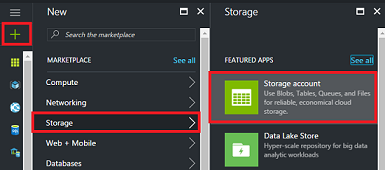
\includegraphics{/Users/azureimages/1}
\end{figure}
3. Enter a unique name for your storage account. Name must be of 3-24 \indent characters in length and may contain numbers and lowercase letters only. 
\begin{figure}[H]
	\centering
	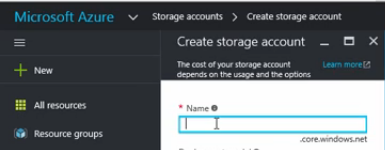
\includegraphics{/Users/azureimages/2}
\end{figure}
\clearpage
4. Select the deployment model option as \textbf{Resource Manager} . Blob \indent storage accounts can only be created using this particular option. 
\begin{figure}[H]
	\centering
	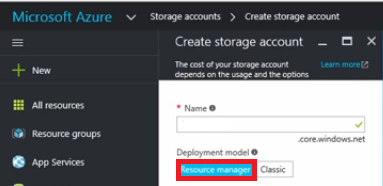
\includegraphics{/Users/azureimages/3}
\end{figure}
5. Change the type of storage account from General purpose to \textbf{Blob \indent Storage}. By default it is General purpose.
\begin{figure}[H]
	\centering
	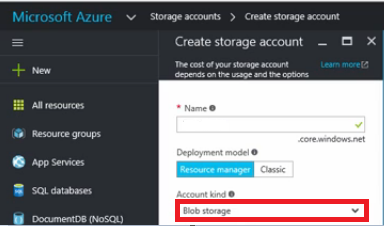
\includegraphics{/Users/azureimages/4}
\end{figure}
\clearpage
6. Now for \textbf{Performance} and \textbf{Replication} wise we will leverage the \indent default options for this demo.
\begin{figure}[H]
	\centering
	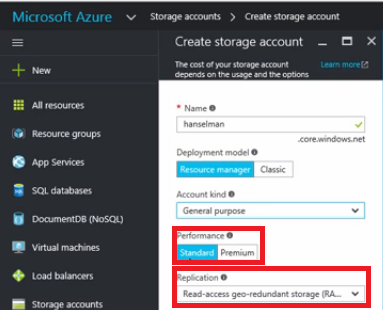
\includegraphics{/Users/azureimages/5}
\end{figure}
7. Leave the remaining fields default and hit the pin to dashboard button \indent at the bottom of your screen. Finally click the \textbf{Create} button to create \indent the storage account.  


	
\end{document}